\documentclass[11pt]{beamer}
\usepackage[utf8]{inputenc}
\usepackage[T1]{fontenc}
\usepackage{lmodern}
\usetheme{AnnArbor}
\begin{document}
	\author{A R Bathri Narayanan}
	\title{Search on Superconducting Qubits}
	\subtitle{International Young Quantum Meet 2024}
	%\logo{}
	\institute{UM-DAE Centre for Excellence in Basic Sciences}
	\date{September 17, 2024}
	\subject{}
	%\setbeamercovered{transparent}
	%\setbeamertemplate{navigation symbols}{}
	\begin{frame}[plain]
		\maketitle
	\end{frame}
	
	\begin{frame}
		\frametitle{Introduction to the talk}
		Qubits can be realised in a lot of ways, examples include
		\begin{enumerate}
			\item  Ion trap quantum computing
			\item NMR quantum computing
			\item Optical photon quantum computing to name a few.
		\end{enumerate}
	My talk will be focused more on Superconducting qubits and applying it to model a theoretical problem.
	\end{frame}
	
		\begin{frame}
		\frametitle{How do you build Superconducting Qubits}
		By using so called "Artificial atoms". You cool a LC circuit to the material's critical temperature, into it's superconducting phase.\\
		\begin{center}
		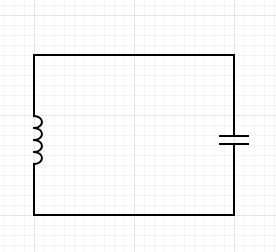
\includegraphics[width=3 cm]{sc1.png}
		\end{center}
		Where,
		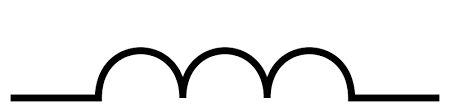
\includegraphics[width=1 cm]{sc2.png} means Inductor and 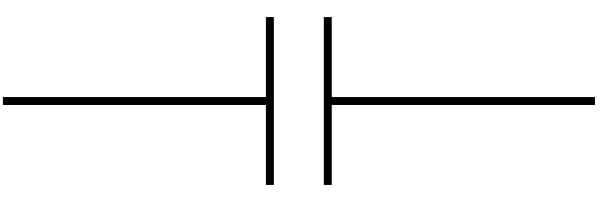
\includegraphics[width=1 cm]{sc3.jpg} means Capacitor. The Hamiltonian of this circuit is given by
		\[H=\frac{\hat{Q}}{2C}+\frac{\hat{\Phi}}{2L}=\hbar\omega(aa^{\dagger}+\frac{1}{2})\]
		\end{frame}
		
				\begin{frame}
			\frametitle{Issues with simple superconducting qubits}
			Energy levels of the circuit mimic a linear Harmonic oscillator
			\begin{center}
			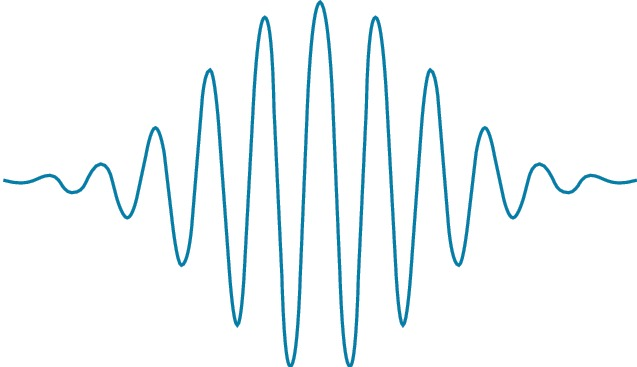
\includegraphics[width=2 cm]{sc5.jpg}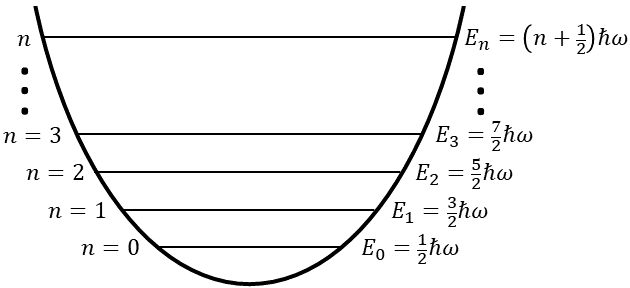
\includegraphics[width=5 cm]{sc4.png}
			\end{center}
			This can't be an ideal two qubit system as all energy levels are equally spaced. But how do we modify the energy levels?\\
			Enter \textbf{Josephson Junctions} !!
			\begin{center}
				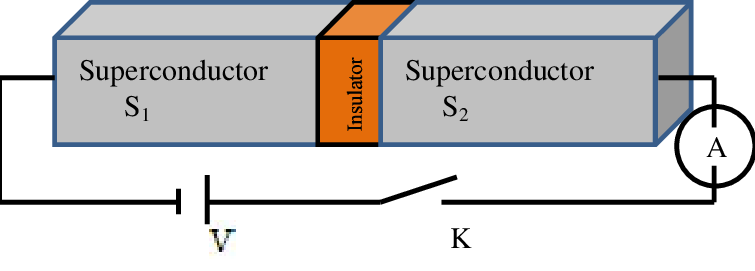
\includegraphics[width=5 cm]{sc6.png}
			\end{center}

		\end{frame}
	
		\begin{frame}
		\frametitle{How can you modify Superconducting Qubits (Josephson Junctions and dc-SQUIDs)}
		Josephson Junctions are represented by 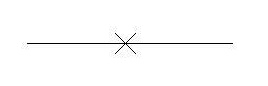
\includegraphics[width=1 cm]{sc7.png}. I am not focusing more on the derivation of V, I and L of Josephson Junctions, I just mention it here. Interested can refer to Feynman lectures volume 3 last chapter.
		\[V_J=\frac{\Phi_0}{2\pi}\frac{d\varphi_J}{dt}\]
		\[I_J=I_c sin \varphi_J\]
		\[L_J=\frac{\phi_J}{I_csin(2\pi\phi_J/\phi_0)}=\frac{\phi_0\varphi_J}{2\pi I_c sin\varphi_J}\]
		The circuit can be drawn like\\
		\begin{center}
			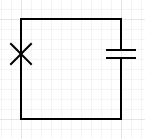
\includegraphics[width=2cm]{sc8.png}
		\end{center}
	

	\end{frame}
	
	\begin{frame}
		\frametitle{Analog gravity using superconducting qubits}
		We construct an infinite circuit like
		\begin{center}
			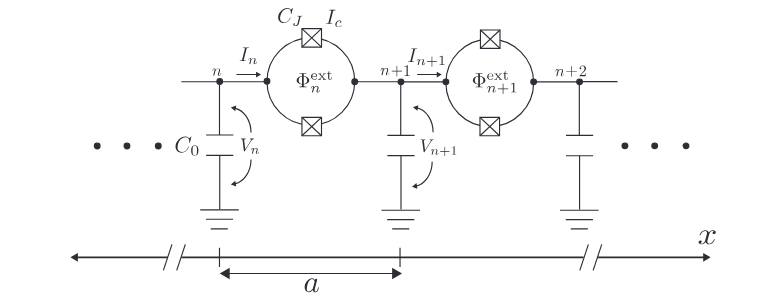
\includegraphics[width=8 cm]{sc9.png}
		\end{center}
		Now, we apply Kirchoff law and Faraday's law as
		\[I_n - I_{n+1}=\frac{dQ_{n+1}}{dt}\]
		\[V_n-V_{n+1}=\frac{\Phi_0}{2\pi}\frac{d\varphi_{Jn}}{dt}\]
	\end{frame}
	
		\begin{frame}
		\frametitle{Obtaining the Lagrangian and Hamiltonian}
Plugging in the formulas obtained for Josephson junctions, we can obtain the current entering the nth unit cell as
\[I_n=2 C_J \frac{\Phi_0}{2\pi}\frac{d^2\varphi_{Jn}}{dt^2}+2I_ccos\bigg(\frac{\pi \Phi^ext_n}{\Phi_0}\bigg)sin\varphi_{Jn}\]
	\end{frame}
	
		\begin{frame}
		\frametitle{Conclusions}
		So in this talk, we have discussed about
		\begin{enumerate}
			\item A brief introduction to Superconducting qubits
			\item  Construction of superconducting qubits
			\item  A brief application of superconducting qubits in Analogue Gravity and Hawking radiation.
			
		\end{enumerate}
	\end{frame}
	
			\begin{frame}
		\frametitle{Acknowledgements}
		I would like to thank the following people for guiding me in the right direction
		\begin{enumerate}
			\item Prof. R Nagarajan, Emeritus professor, UM-DAE Centre for Excellence in Basic Sciences
			\item Prof. Sudhir Ranjan Jain, Adjunct faculty, UM-DAE Centre for Excellence in Basic Sciences
			\item Prof. Ujjwal Sen, Professor-H, Harish-Chandra Research institute
			\item  Prof. Amarendra Kumar Sarma, Professor, IIT Guwahati
		\end{enumerate}
	\end{frame}
	
	\begin{frame}
		\begin{center}
			\LARGE\textbf{Thank You !!}
		\end{center}
	
	\end{frame}
\end{document}